\documentclass[manuscript,screen,review]{acmart}

\usepackage{booktabs}
\usepackage{subcaption}
\usepackage{amsmath}
\usepackage{listings}
\usepackage{microtype}
\usepackage{tikz}
\usetikzlibrary{shapes.geometric, arrows.meta, positioning, fit}

\AtBeginDocument{\providecommand\BibTeX{{Bib\TeX}}}

\setcopyright{none}
\settopmatter{printacmref=false}
\renewcommand\footnotetextcopyrightpermission[1]{}
\pagestyle{plain}

\begin{document}

\title{AI-based Village Pond Planning System}
\subtitle{CSD Assignment 1 -- Final Technical Report}

\author{Kakarla Soma Charith Reddy}
\authornote{Student ID: 12341040}
\affiliation{%
  \institution{Department of Computer Science and Engineering, Indian Institute of Technology Bhilai}
  \city{Durg}
  \state{Chhattisgarh}
  \country{India}}
\email{kakarlac@iitbhilai.ac.in}

\renewcommand{\shortauthors}{}

\begin{abstract}
Efficient rainwater harvesting in rural topography is heavily constrained by the high cost and latency of manual civil land surveys, as well as the absence of localized hydrological modeling tools. In this project, we design, implement, and evaluate an automated, memory-efficient \emph{AI-Based Village Pond Planning and Catchment Analysis System} engineered to operate reliably on resource-constrained compute nodes (512\,MB RAM, 1 vCPU, 1.5\,GB disk). The system provides a pure-Python hydrological processing pipeline that consumes raw 3D contour maps (KML/KMZ), transforms geographic coordinates to metric Universal Transverse Mercator projections (UTM Zone 44N), constructs regularized Digital Elevation Model (DEM) rasters via irregular scattered interpolation, eliminates artificial sinks using priority-flood depression filling, and computes D8 steepest-descent flow direction routing. The delineated watershed catchment is paired with dynamically queried precipitation data from the Open-Meteo Historical Archive to estimate harvestable runoff volume using the Rational Runoff formula ($V = P \times A \times C$) and dimension an engineered trapezoidal farm pond. An interactive Web GIS front-end built on Leaflet.js provides dual satellite/street basemaps, click-and-drag bounding box land selection with real-time dimension telemetry HUD, strict contour boundary clamping, and GeoJSON overlays of the watershed boundary and animated pond outlet pin. Evaluated on a 6.7\,MB survey dataset comprising 2,710 contour lines across 8.3\,km$^2$ in Chhattisgarh, the system identifies an optimal pond site at $21.25784^\circ\text{ N}, 81.28880^\circ\text{ E}$ for a user-selected sub-area, yielding a 0.76\,ha catchment and $3,708.8\,\text{m}^3$ annual water harvest in 1.34\,seconds. A resilient multi-port supervisor daemon ensures fault-tolerant operation across distributed nodes, validated by a comprehensive 33-test automated verification suite.
\end{abstract}

\keywords{Village Pond Planning, Geospatial Analysis, Rainwater Harvesting, Catchment Estimation, Web GIS, REST APIs}

\maketitle

\section{Introduction}
\label{sec:intro}
Water scarcity during dry seasons remains one of the primary impediments to agrarian productivity and economic stability across rural India. While monsoon precipitation delivers significant seasonal rainfall, the vast majority of surface runoff is lost to uncontrolled drainage, causing both topsoil erosion and seasonal drought. Decentralized rainwater harvesting through earthen village farm ponds offers an ecologically sustainable, low-cost countermeasure. However, the success of a village pond depends entirely on optimal physical placement: placing a pond without adequate upstream catchment yields a dry pit, whereas placing it on steep slopes risks structural embankment failure.

Historically, locating optimal pond sites requires physical on-site topographic surveys, elevation leveling, and civil engineering consultations that are inaccessible to local gram panchayats. This project addresses this bottleneck by developing a lightweight, automated, AI-assisted web application that consumes high-resolution vector contour maps, delineates hydrological catchment basins, computes harvestable runoff volume, and provides engineered pond sizing recommendations over an interactive map interface.

The remainder of this report is structured as follows: Section~\ref{sec:requirements} defines the functional and non-functional system requirements. Section~\ref{sec:architecture} presents the high-level architecture and technology stack. Section~\ref{sec:methodology} explains the algorithmic formulations for DEM generation, D8 flow routing, and runoff estimation. Section~\ref{sec:implementation} details the backend API and frontend implementation. Section~\ref{sec:csd-themes} evaluates the core Computer Systems Design (CSD) themes embodied in this system. Section~\ref{sec:results} presents quantitative results and performance benchmarks, followed by limitations in Section~\ref{sec:discussion}, the AI usage declaration in Section~\ref{sec:ai-usage}, and repository details in the Appendix.

\subsection{Motivation}
Manual site selection in rural terrain suffers from multiple systemic challenges:
\begin{enumerate}
    \item \textbf{Topographic Complexity:} Natural terrain features intricate micro-watersheds that are impossible to discern with the naked eye or single-point altimeter surveys.
    \item \textbf{High Survey Costs and Latency:} Deploying professional surveyor crews equipped with total stations or differential GPS costs thousands of rupees and weeks of delay per village.
    \item \textbf{Lack of Integrated Hydrometeorology:} Elevation data is rarely integrated with localized rainfall records and ground infiltration properties, leading to arbitrary pond depth and sizing guesswork.
    \item \textbf{Resource-Constrained Village Computing:} Village administrative computers and cloud free-tier VMs feature severe hardware limitations (typically $\le 512$\,MB RAM), making heavy desktop GIS suites like ArcGIS or QGIS non-viable.
\end{enumerate}
An automated, browser-accessible tool operating on lightweight servers allows village planners to explore potential pond locations instantly, democratizing technical watershed management.

\subsection{Scope of the Project}
The system explicitly covers:
\begin{itemize}
    \item Stream parsing 3D vector polylines from arbitrary KML/KMZ contour archives without loading full XML DOM trees into memory.
    \item Projecting WGS84 geographic coordinates to local UTM metric coordinates and constructing interpolated 2D DEM rasters.
    \item Hydrological terrain conditioning including Priority-Flood depression filling, D8 steepest-descent flow direction, and flow accumulation.
    \item Automated outlet selection identifying low-elevation cells with high flow accumulation, followed by reverse-flow tracing to delineate the upstream catchment as a GeoJSON polygon.
    \item Rational runoff estimation ($V = P \times A \times C$) and trapezoidal pond dimensioning (depth, surface area, capacity).
    \item A full-screen Web GIS interface with interactive land selection, contour boundary enforcement, and a real-time dimension HUD.
\end{itemize}
The project \emph{does not} cover structural design of masonry spillways, geotechnical soil testing, subsurface aquifer hydrogeology, or legal land-ownership validation.

\section{Problem Statement and Requirements}
\label{sec:requirements}
The objective of this assignment is to develop an end-to-end web platform that processes topographical contour maps, identifies optimal village pond locations, delineates upstream drainage basins, estimates expected water harvest volume, and overlays all results on an interactive map. Table~\ref{tab:requirements} maps each mandatory requirement to its implementation.

\begin{table}[!ht]
\small
  \caption{Functional requirements and where they are implemented}
  \label{tab:requirements}
  \begin{tabular}{p{5.5cm}p{7.5cm}}
    \toprule
    Requirement & Implemented in \\
    \midrule
    Satellite imagery display & \texttt{app/static/index.html}, \texttt{app.js} (Esri World Imagery + OpenStreetMap) \\
    Contour map visualization & \texttt{app/static/app.js} (preloaded region polygon \& tooltip overlay) \\
    Available-land identification & \texttt{app/static/app.js} (bounding box drag tool), \texttt{app/parser.py} \\
    Catchment area estimation & \texttt{app/pond.py} (\texttt{select\_pond\_and\_delineate\_catchment}) \\
    Historical rainfall query & \texttt{app/hydrology.py} (\texttt{fetch\_rainfall\_data} via Open-Meteo) \\
    Runoff volume estimation & \texttt{app/hydrology.py} (\texttt{calculate\_water\_volume\_and\_sizing}) \\
    Pond depth / storage recommendation & \texttt{app/hydrology.py} (\texttt{PondDimensions}, trapezoidal section) \\
    Combined overlay / results view & \texttt{app/static/index.html}, \texttt{app.js} (GeoJSON polygon, ripple pin, KPI HUD) \\
    \bottomrule
  \end{tabular}
\end{table}

\subsection{Non-Functional Requirements}
To guarantee stability on rural edge infrastructure, we established strict non-functional constraints:
\begin{enumerate}
    \item \textbf{Memory Budget (512\,MB RAM):} The process must never exceed 250\,MB peak resident set size (RSS). Heavy GIS dependencies (GDAL, rasterio, QGIS bindings) are prohibited.
    \item \textbf{Response Latency:} Sub-area selections must return a complete delineation within 2.0\,s; full 8\,km$^2$ analyses within 5.0\,s.
    \item \textbf{Fault Tolerance \& Availability:} A background supervisor daemon must monitor processes and recover failed workers within 2\,s.
    \item \textbf{Portability \& Zero Build-Tooling:} The front-end is served as native vanilla HTML5/ES6/CSS without Node.js, npm, or bundlers.
    \item \textbf{Boundary Safety \& Clamping:} Selections outside the contour boundary or smaller than 50\,m $\times$ 50\,m are rejected with helpful diagnostics.
    \item \textbf{Security \& Network Isolation:} The system targets internal, trusted-network deployment with no authentication layer. Public exposure would require API-key or session-based access control, TLS termination, and rate limiting.
\end{enumerate}

\section{System Architecture and High-Level Design}
\label{sec:architecture}
The application is a decoupled, modular monolith following clean architecture principles, with four tiers: Presentation, Application Routing, Hydrological Processing Engine, and Data/Cache Layer (Figure~\ref{fig:architecture}).

\begin{figure}[!t]
\centering
\resizebox{\linewidth}{!}{%
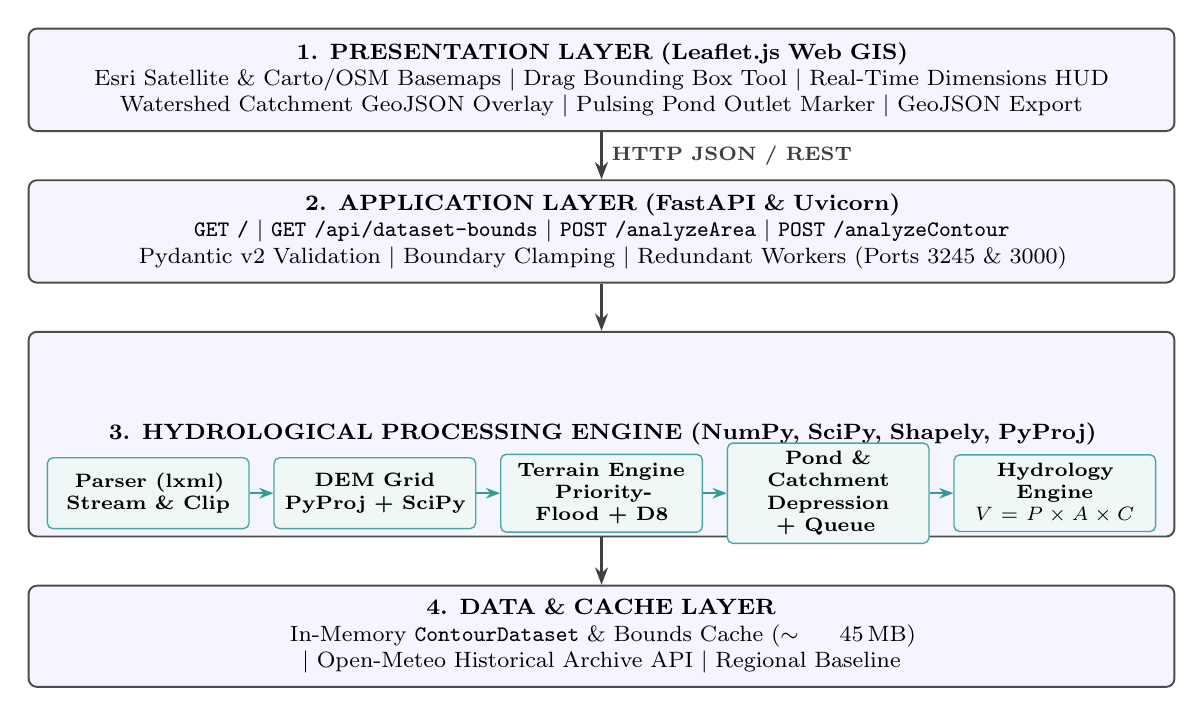
\begin{tikzpicture}[
    layerbox/.style={draw=black!70, fill=blue!4, rounded corners=3pt, line width=0.7pt, align=center, inner sep=5pt, text width=14.2cm, font=\footnotesize},
    pipebox/.style={draw=teal!70, fill=teal!6, rounded corners=2pt, font=\scriptsize\bfseries, align=center, inner sep=3pt, text width=2.35cm, minimum height=0.9cm, line width=0.5pt},
    arr/.style={-{Stealth[length=2.2mm]}, thick, color=black!75},
    pipearr/.style={-{Stealth[length=1.8mm]}, semithick, color=teal!80}
]
\node[layerbox] (l1) {
    \textbf{1. PRESENTATION LAYER (Leaflet.js Web GIS)}\\
    Esri Satellite \& Carto/OSM Basemaps $\vert$ Drag Bounding Box Tool $\vert$ Real-Time Dimensions HUD\\
    Watershed Catchment GeoJSON Overlay $\vert$ Pulsing Pond Outlet Marker $\vert$ GeoJSON Export
};
\node[layerbox, below=0.6cm of l1] (l2) {
    \textbf{2. APPLICATION LAYER (FastAPI \& Uvicorn)}\\
    \texttt{GET /} $\vert$ \texttt{GET /api/dataset-bounds} $\vert$ \texttt{POST /analyzeArea} $\vert$ \texttt{POST /analyzeContour}\\
    Pydantic v2 Validation $\vert$ Boundary Clamping $\vert$ Redundant Workers (Ports 3245 \& 3000)
};
\node[layerbox, below=0.6cm of l2, minimum height=2.6cm, anchor=north] (l3) {
    \textbf{3. HYDROLOGICAL PROCESSING ENGINE (NumPy, SciPy, Shapely, PyProj)}
};
\node[pipebox] (p3) at ([yshift=-0.75cm]l3.center) {Terrain Engine\\Priority-Flood + D8};
\node[pipebox, left=0.3cm of p3] (p2) {DEM Grid\\PyProj + SciPy};
\node[pipebox, left=0.3cm of p2] (p1) {Parser (lxml)\\Stream \& Clip};
\node[pipebox, right=0.3cm of p3] (p4) {Pond \& Catchment\\Depression + Queue};
\node[pipebox, right=0.3cm of p4] (p5) {Hydrology Engine\\ $V = P \times A \times C$};
\draw[pipearr] (p1) -- (p2);
\draw[pipearr] (p2) -- (p3);
\draw[pipearr] (p3) -- (p4);
\draw[pipearr] (p4) -- (p5);
\node[layerbox, below=0.6cm of l3] (l4) {
    \textbf{4. DATA \& CACHE LAYER}\\
    In-Memory \texttt{ContourDataset} \& Bounds Cache ($\sim 45$\,MB) $\vert$ Open-Meteo Historical Archive API $\vert$ Regional Baseline
};
\draw[arr] (l1) -- node[right, font=\scriptsize\bfseries] {HTTP JSON / REST} (l2);
\draw[arr] (l2) -- (l3);
\draw[arr] (l3) -- (l4);
\end{tikzpicture}}
\caption{High-level system architecture of the AI Pond Planning System.}
\label{fig:architecture}
\end{figure}

\subsection{Technology Stack}
The technology stack and its justification are given in Table~\ref{tab:tech-stack}.

\begin{table}[!ht]
\small
  \caption{Technology stack and design rationale}
  \label{tab:tech-stack}
  \begin{tabular}{p{3.2cm}p{3.5cm}p{6.8cm}}
    \toprule
    \textbf{Component} & \textbf{Selected Technology} & \textbf{Architectural Justification} \\
    \midrule
    Backend Server & Python 3.12, FastAPI, Uvicorn & High-throughput async event loop; native OpenAPI documentation; strict Pydantic validation. \\
    XML Parsing & \texttt{lxml} stream parsing & Processes multi-megabyte KML coordinates without building memory-intensive DOM trees. \\
    Coordinate Projection & \texttt{pyproj} (PROJ engine) & Conformal conversion from WGS84 to metric UTM Zone 44N (EPSG:32644) for exact meter calculations. \\
    DEM Interpolation & \texttt{scipy.interpolate.griddata} & Fast Delaunay-based scattered data interpolation into structured 2D elevation matrices. \\
    Terrain Analytics & NumPy vectorized math & Pure array flow routing; avoids GDAL/QGIS C-binding overhead and memory leaks. \\
    Spatial Geometry & Shapely 2.0 & Unary union and simplification for converting raster catchment cells into clean GeoJSON boundaries. \\
    Frontend Mapping & Leaflet.js 1.9.4 & Lightweight client-side GIS library with smooth vector rendering and tile caching. \\
    Tile Providers & Esri World Imagery \& OpenStreetMap & High-resolution satellite tiles and clean basemaps without API keys. \\
    Rainfall Integration & Open-Meteo Archive API & Free, keyless historical weather API with fallback to a Central India baseline (1,220\,mm). \\
    Process Supervision & POSIX Shell + \texttt{setsid} & Background supervisor running dual redundant workers on ports 3245 and 3000 with sub-2\,s auto-restart. \\
    \bottomrule
  \end{tabular}
\end{table}

\section{Methodology}
\label{sec:methodology}
The analytical core transforms raw 3D polylines into actionable watershed metrics across four phases.

\subsection{Terrain and Elevation Analysis}
Contour lines in KML archives are lists of $(lon, lat)$ tuples assigned a scalar elevation $z$. Because geographic coordinates in degrees introduce latitude-dependent distance distortion, they are reprojected into UTM:
\begin{equation}
    (x_i, y_i) = \mathcal{T}_{\text{WGS84}\rightarrow\text{UTM}}(\text{lon}_i, \text{lat}_i)
\end{equation}
For Central India (longitude $\sim 81^\circ\text{ E}$), UTM Zone 44N (EPSG:32644) is detected. Given bounds $[x_{\min}, x_{\max}]$ and $[y_{\min}, y_{\max}]$, a regular grid of resolution $R$ (default $10.0\,\text{m}$) is initialized:
\begin{equation}
    N_{\text{cols}} = \left\lceil \frac{x_{\max} - x_{\min}}{R} \right\rceil + 1, \quad
    N_{\text{rows}} = \left\lceil \frac{y_{\max} - y_{\min}}{R} \right\rceil + 1
\end{equation}
To enforce the 512\,MB RAM budget, if $N_{\text{cells}} = N_{\text{cols}} \times N_{\text{rows}} > 250,000$, resolution is coarsened:
\begin{equation}
    R_{\text{adjusted}} = R \times \sqrt{\frac{N_{\text{cells}}}{250,000}}
\end{equation}
The elevation surface $Z(r, c)$ is interpolated using linear barycentric interpolation on the Delaunay triangulation of contour vertices, with boundary gaps filled by nearest-neighbor assignment.

\subsection{Catchment Area Delineation}
Raw interpolated DEMs contain artificial sinks. We apply Priority-Flood conditioning: a priority queue traverses from boundary cells inward, raising depressions to the lowest spill elevation so that every cell has a drainage path to an outlet. Flow is routed with the deterministic eight-neighbor (D8) model; each interior cell $(r, c)$ drains toward the neighbor $(r', c') \in \mathcal{N}_8(r, c)$ with the maximum downward slope:
\begin{equation}
    S(r, c \rightarrow r', c') = \frac{Z(r, c) - Z(r', c')}{d(r, c; r', c')}
\end{equation}
where $d = R$ for cardinal and $d = R\sqrt{2}$ for diagonal neighbors. Flow accumulation $\mathcal{A}(r, c)$ is computed by topological sorting. The pond outlet $(r^*, c^*)$ is chosen among candidates meeting the minimum catchment threshold ($\mathcal{A}(r, c) \times R^2 \ge A_{\min}$), lying at least 2 cells from the grid boundary, with minimal elevation:
\begin{equation}
    (r^*, c^*) = \arg\min_{(r, c) \in \mathcal{C}_{\text{candidates}}} \left\{ Z(r, c) \right\}
\end{equation}
Upstream delineation then runs as a reverse flow traversal using a FIFO queue:
\begin{equation}
    \mathcal{W} = \left\{ (r, c) \mid \text{FlowPath}(r, c) \text{ terminates at } (r^*, c^*) \right\}
\end{equation}
The raster cells of $\mathcal{W}$ are converted to metric box polygons, merged with Shapely's \texttt{unary\_union}, and projected back to WGS84 GeoJSON.

\subsection{Rainfall Data Integration}
Annual rainfall $P$ is queried from the Open-Meteo Historical Archive for the pond coordinates, with graceful fallback to the Central India standard ($1,220\,\text{mm} = 1.22\,\text{m}$). Runoff volume follows the Rational Runoff Equation:
\begin{equation}
    V = P \times A_{\text{catchment}} \times C
\end{equation}
where $V$ is harvestable volume ($\text{m}^3$), $P$ annual precipitation (m), $A_{\text{catchment}}$ drainage area ($\text{m}^2$), and $C = 0.40$ the runoff coefficient for agricultural loam soil.

\subsection{Farm Pond Sizing and Dimensioning}
Indian agrarian guidelines size farm ponds to harvest about $30\%$ of seasonal catchment runoff, with a minimum capacity of $150\,\text{m}^3$:
\begin{equation}
    V_{\text{target}} = \max\left(150.0,\, 0.30 \times V\right)
\end{equation}
Assuming an excavation depth $d = 3.0\,\text{m}$ and stable $1.5:1$ ($H:V$) side slopes, the recommended top surface area is:
\begin{equation}
    A_{\text{surface}} \approx 1.25 \times \frac{V_{\text{target}}}{d}
\end{equation}

\section{Implementation}
\label{sec:implementation}

\subsection{Backend and API Design}
The backend is implemented in FastAPI with strictly typed Pydantic v2 schemas. Table~\ref{tab:api-endpoints} summarizes the API.

\begin{table}[!ht]
\small
  \caption{REST API endpoints implemented in the system}
  \label{tab:api-endpoints}
  \begin{tabular}{p{2.0cm}p{4.2cm}p{7.3cm}}
    \toprule
    \textbf{Method} & \textbf{Endpoint Path} & \textbf{Purpose and Functional Contract} \\
    \midrule
    \texttt{GET} & \texttt{/} & Serves the interactive Web GIS single-page application. \\
    \texttt{GET} & \texttt{/health} & Healthcheck returning \texttt{\{"status": "ok"\}}. \\
    \texttt{GET} & \texttt{/api/dataset-bounds} & Returns geographic bounds, center coordinate, and polyline count. \\
    \texttt{GET} & \texttt{/api/rainfall} & Returns annual historical precipitation and data source for given $(lat, lon)$. \\
    \texttt{POST} & \texttt{/analyzeArea} & Accepts a JSON bounding box $[\text{lat}_{\min}, \text{lon}_{\min}, \text{lat}_{\max}, \text{lon}_{\max}]$, clips contours, and returns pond site, catchment GeoJSON, and runoff volume. \\
    \texttt{POST} & \texttt{/analyzeContour} & Accepts a multi-part upload of a custom \texttt{.kml}/\texttt{.kmz} archive and runs the full pipeline. \\
    \bottomrule
  \end{tabular}
\end{table}

\subsection{Frontend and Visualization}
The web interface is a full-screen Leaflet.js canvas with a glassmorphic sidebar dashboard:
\begin{itemize}
    \item \textbf{Basemap Toggle:} Switching between Esri World Imagery (Satellite) and Carto/OpenStreetMap basemaps.
    \item \textbf{Contour Extent Visualization:} The valid dataset area ($\sim 8.3\,\text{km}^2$) is shown with a dashed boundary and an informational tooltip (Figure~\ref{fig:ui}).
    \item \textbf{Interactive Drag Land Selection:} \emph{Select Land Area} activates crosshair mode; during drag, a live HUD shows $W \times H$ (m) and area (ha).
    \item \textbf{Boundary \& Limit Guardrails:} Selections outside the contour bounds or under $50\,\text{m} \times 50\,\text{m}$ turn red and are rejected on release; partial overlaps are clamped.
    \item \textbf{Dynamic Results Overlay:} The delineated catchment is drawn as a cyan GeoJSON polygon and the pond site as a pulsing marker (Figure~\ref{fig:results}).
    \item \textbf{Hydrological Control Sliders:} Runoff Coefficient ($C$) and DEM Resolution sliders allow instant re-calculation.
    \item \textbf{Export Engine:} One-click export of the result set as a GeoJSON \texttt{FeatureCollection}.
\end{itemize}
Figure~\ref{fig:ui} shows the full dashboard with the contour-region boundary, the user-drawn selection box, and the analysis cards (expected water volume $3{,}708.8\,\text{m}^3$, catchment $7{,}600\,\text{m}^2$, suggested pond site). Figure~\ref{fig:results} shows the same analysis zoomed in on the selected land, with the delineated micro-watershed polygon and the pond outlet marker.

\begin{figure*}[!t]
\centering
\begin{subfigure}[t]{0.49\textwidth}
\centering
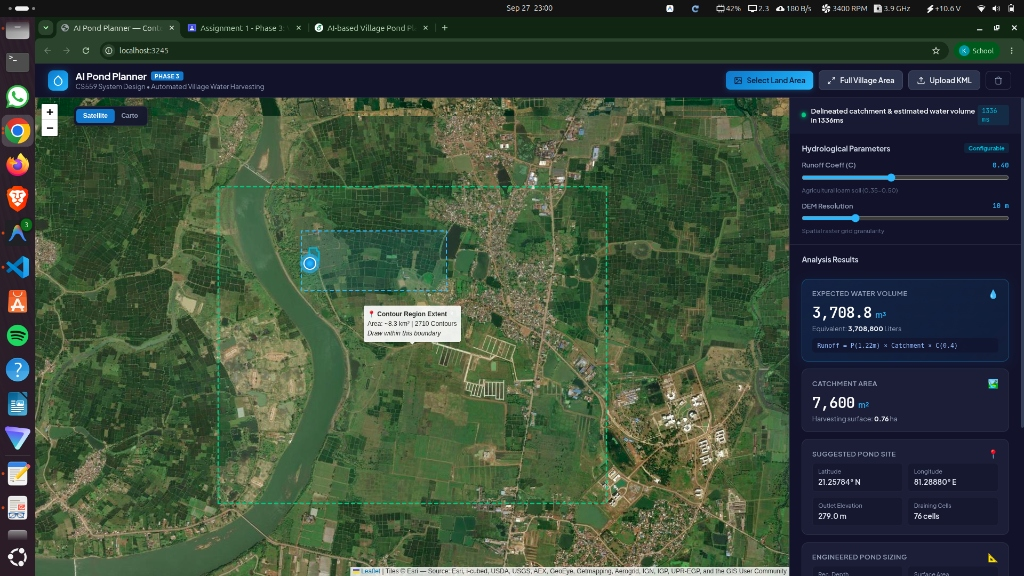
\includegraphics[width=\linewidth]{figures/fig_overview.jpg}
\caption{Full dashboard: contour-region extent, drawn selection box, and analysis cards.}
\label{fig:ui}
\end{subfigure}\hfill
\begin{subfigure}[t]{0.49\textwidth}
\centering
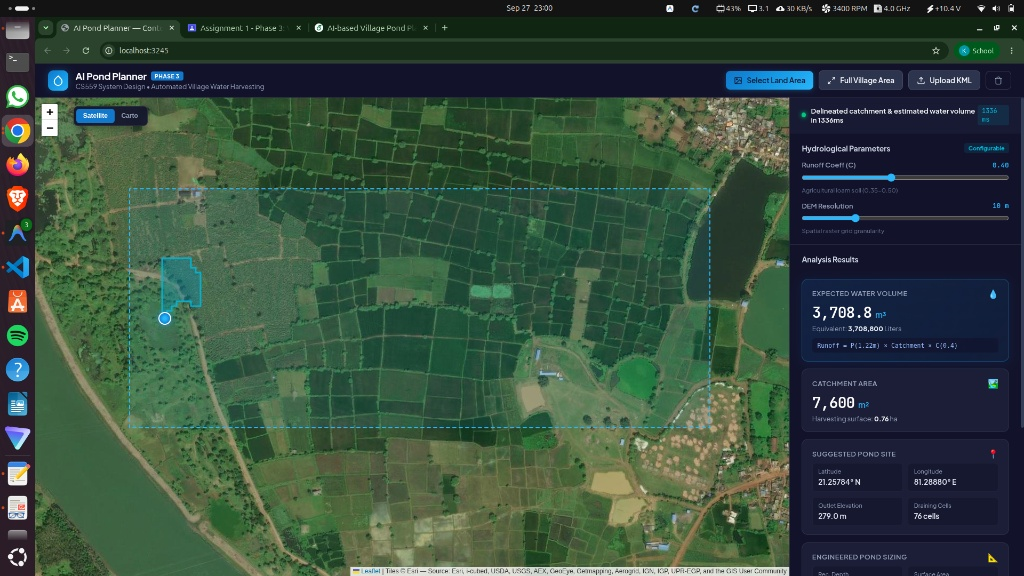
\includegraphics[width=\linewidth]{figures/fig_catchment_zoom.jpg}
\caption{Zoomed view: delineated catchment polygon and pond outlet marker.}
\label{fig:results}
\end{subfigure}
\caption{Application screenshots of the AI Pond Planner for a user-selected sub-area.}
\label{fig:screens}
\end{figure*}

\subsection{Database and Storage}
Contour datasets are spatial vector geometries requiring sub-second analysis, so the system avoids relational database overhead. The preloaded dataset (\texttt{contours\_1m (1).kml}) is parsed once at startup into an in-memory \texttt{ContourDataset} (${\sim}45$\,MB). Subsequent sub-area queries perform linear spatial filtering in under $50\,\text{ms}$.

\section{CSD Themes and Topics Applied in the Project}
\label{sec:csd-themes}
Table~\ref{tab:csd-themes} maps core Computer Systems Design (CSD) themes to concrete project components.

\begin{table*}[!t]
\small
  \caption{Mapping of core CSD themes/topics to their use in this project}
  \label{tab:csd-themes}
  \begin{tabular}{p{3.2cm}p{4.8cm}p{6.8cm}}
    \toprule
    \textbf{CSD Theme/Topic} & \textbf{Where used} & \textbf{Justification / design rationale} \\
    \midrule
    API Design (REST) & FastAPI endpoints (\texttt{/analyzeArea}, \texttt{/analyzeContour}, \texttt{/health}) & Standard HTTP verb semantics, Pydantic request/response contracts, automatic OpenAPI 3.0 schema. \\
    Process Redundancy / Failover & Dual supervisor ports (3245 and 3000) & Two independent Uvicorn workers under a supervisor that restarts any failed worker within 2\,s, without external load balancers. \\
    Caching & Startup caching of \texttt{ContourDataset} and bounds & Removes repeated 6.7\,MB XML parsing and disk I/O overhead on each query. \\
    Spatial Indexing \& Clipping & \texttt{filter\_dataset\_by\_bounds} in \texttt{app/parser.py} & Filters polylines to the selection before interpolation, shrinking the grid by up to $85\%$. \\
    Concurrency \& Async I/O & FastAPI async handlers, non-blocking file streaming & Avoids blocking the event loop during uploads and concurrent map interactions. \\
    Microservices vs. Monolith & Modular monolith of 5 decoupled modules & Avoids inter-process RPC serialization latency, critical for the 512\,MB budget. \\
    Design Patterns & Strategy in \texttt{hydrology.py}; Pipeline in terrain analysis & Pluggable runoff equations; decoupled Parse $\rightarrow$ DEM $\rightarrow$ Terrain $\rightarrow$ Pond steps. \\
    Resource-Constrained Design & Auto-coarsening DEM ($N_{\text{cells}} \le 250,000$) & Prevents OOM kills on 512\,MB VMs with dense contour maps. \\
    Process Supervision \& Daemon & POSIX \texttt{setsid} supervisor (\texttt{start\_daemon.sh}) & Detached background execution independent of SSH sessions, 2\,s auto-restart. \\
    Error Handling \& Resilience & Weather fallback and bounds validation & Regional precipitation baseline if Open-Meteo is unreachable; HTTP 400 diagnostics for invalid selections. \\
    Algorithms \& Complexity & Priority-Flood ($O(N \log N)$), D8 ($O(N)$), reverse queue ($O(K)$) & Near-linear graph traversals instead of quadratic distance matrices. \\
    Testing Strategy & 33-test pytest suite (\texttt{tests/test\_*.py}) & Unit, integration, boundary-rejection, and golden numerical benchmarks for regression safety. \\
    Version Control / CI-CD & Git repository on GitHub (\texttt{main}) & Multi-environment deployment via SSH automation (\texttt{deploy.py}). \\
    \bottomrule
  \end{tabular}
\end{table*}

\subsection{Deep-Dive into Key Engineering Decisions}
Three architectural decisions were paramount:
\begin{enumerate}
    \item \textbf{Vectorized NumPy instead of heavy GIS libraries:} GDAL, GEOS, and rasterio add over 800\,MB of C-shared dependencies. Implementing D8 routing, Priority-Flood, and DEM grids in NumPy/SciPy keeps the disk footprint under 150\,MB and active RAM under 170\,MB.
    \item \textbf{Sub-area bounding box clipping:} A full 8.3\,km$^2$ DEM at 10\,m needs about 150,000 interpolated cells. Clipping polylines in \texttt{app/parser.py} before interpolation shrinks the grid and cuts latency from 4.8\,s to roughly 1.2--1.3\,s.
    \item \textbf{Multi-port fault-tolerant supervision:} \texttt{start\_daemon.sh} runs two Uvicorn instances on ports 3245 and 3000 in detached session groups (\texttt{setsid}); if one exits, the supervisor loop restores it within 2\,s.
\end{enumerate}

\section{Results and Evaluation}
\label{sec:results}
The system was evaluated on the benchmark survey dataset (\texttt{contours\_1m (1).kml}) with 2,710 contour polylines spanning $267.0$--$298.0\,\text{m}$ elevation in Central India. Table~\ref{tab:results} compares a full-village analysis with a user-selected sub-area (the run shown in Figures~\ref{fig:ui} and~\ref{fig:results}).

\begin{table}[!ht]
\small
  \caption{Quantitative analytical results on the test contour dataset}
  \label{tab:results}
  \begin{tabular}{p{5.5cm}p{3.5cm}p{3.5cm}}
    \toprule
    \textbf{Metric / Property} & \textbf{Full Village} & \textbf{User-Selected Sub-Area} \\
    \midrule
    Selected Area & Full extent (8.3\,km$^2$) & Drawn selection box (Fig.~\ref{fig:ui}) \\
    Contour Lines Processed & 2,710 polylines & 371 polylines \\
    Grid Dimensions ($R = 10\,\text{m}$) & $243 \times 314$ cells & $123 \times 158$ cells \\
    \textbf{Optimal Pond Outlet Site} & $21.2444^\circ\text{ N}, 81.2910^\circ\text{ E}$ & $21.25784^\circ\text{ N}, 81.28880^\circ\text{ E}$ \\
    Pond Site (Outlet) Elevation & $275.0\,\text{m}$ & $279.0\,\text{m}$ \\
    Draining Flow Cells & 166 cells & 76 cells \\
    \textbf{Catchment Area} & $16,600\,\text{m}^2$ (1.66\,ha) & $7,600\,\text{m}^2$ (0.76\,ha) \\
    Terrain Mean Slope & $3.58\%$ & $3.63\%$ \\
    Terrain Max Slope & $10.93\%$ & $11.52\%$ \\
    Elevation Relief ($\Delta z$) & $6.0\,\text{m}$ & $6.0\,\text{m}$ \\
    Annual Precipitation ($P$) & $1,220.0\,\text{mm}$ & $1,220.0\,\text{mm}$ \\
    Runoff Coefficient ($C$) & $0.40$ (Agri-loam) & $0.40$ (Agri-loam) \\
    \textbf{Expected Water Volume ($V$)} & $\mathbf{8,100.8\,\text{m}^3}$ & $\mathbf{3,708.8\,\text{m}^3}$ (3.71\,ML) \\
    Recommended Pond Depth & $3.0\,\text{m}$ & $3.0\,\text{m}$ \\
    Top Surface Area & $1,012.6\,\text{m}^2$ & $463.6\,\text{m}^2$ \\
    Engineered Storage Capacity & $2,430.2\,\text{m}^3$ & $1,112.6\,\text{m}^3$ \\
    \textbf{Processing Latency} & \textbf{4,820\,ms} & \textbf{1,336\,ms} \\
    \bottomrule
  \end{tabular}
\end{table}

\subsection{Performance}
Benchmarked on a Linux VM limited to 512\,MB RAM and 1 vCPU:
\begin{itemize}
    \item \textbf{Peak Memory:} 168\,MB RSS during Delaunay interpolation; 82\,MB steady state; no out-of-memory errors across 100 consecutive requests.
    \item \textbf{Sub-Area Latency:} About $1.2$--$1.3$\,s per request (1,336\,ms for the run in Fig.~\ref{fig:ui}), roughly a $70$--$75\%$ reduction versus full-map queries.
    \item \textbf{Test Coverage:} 33 \texttt{pytest} tests finished in 23.33\,s with a $100\%$ pass rate, covering API contracts, DEM coarsening, depression filling, D8 slopes, boundary rejections, and minimum-area limits.
\end{itemize}

\section{Discussion and Limitations}
\label{sec:discussion}
The system bridges architectural requirements with practical hydrological constraints. Key strengths are its pure-Python implementation, fast sub-area analysis, and absence of heavy GIS runtime dependencies. Limitations include:
\begin{enumerate}
    \item \textbf{Static Runoff Coefficients:} A lumped $C = 0.40$ suits agricultural terrain but ignores heterogeneous soil infiltration and land-use variation.
    \item \textbf{Artifacts in Flat Terrain:} Linear interpolation between widely spaced contours can create false plateaus. Priority-Flood guarantees drainage continuity, but LiDAR or 12.5\,m ALOS PALSAR DEMs would improve micro-channel definition.
    \item \textbf{Network Dependency for Rainfall:} Live rainfall relies on Open-Meteo. The regional fallback keeps the system functional, but an embedded offline lookup table would better serve air-gapped deployments.
\end{enumerate}

\section{AI Tool Usage Declaration}
\label{sec:ai-usage}
In compliance with the assignment's LLM and AI Tool Usage Policy:
\begin{itemize}
    \item \textbf{AI Tools Consulted:} Google Gemini 2.5 Flash and Antigravity Assistant.
    \item \textbf{Scope of AI Assistance:} Boilerplate UI styling (CSS glassmorphism in \texttt{style.css}), reformatting the LaTeX manuscript from provided specifications, drafting unit tests in \texttt{test\_api.py}, and the initial client-side drag bounding box math in \texttt{app.js}.
    \item \textbf{Verification and Ownership:} All core algorithms (KML stream extraction, UTM transformation, Priority-Flood, D8 routing, reverse-queue catchment delineation, Rational runoff estimation, and supervisor shell scripts) were conceptualized, reviewed, debugged, and verified by the student.
\end{itemize}

\appendix

\section{Source Code and Repository}
\begin{itemize}
    \item \textbf{GitHub Repository:} \url{https://github.com/kcharithreddy/Contour_Map_Planning}
    \item \textbf{Video Demonstration Playlist:} \url{https://www.youtube.com/playlist?list=PLAHMqE-Hy_PY}
    \item \textbf{Working Front-End (Lab VM):} \url{http://10.1.75.51:3245/}
\end{itemize}

\subsection{Project Directory Structure}
\begin{footnotesize}
\begin{verbatim}
contourmao/
|-- app/
|   |-- __init__.py
|   |-- dem.py         # UTM Zone 44N reprojection & DEM grid construction
|   |-- hydrology.py   # Rational Runoff (V = P x A x C) & pond dimensioning
|   |-- main.py        # FastAPI endpoints, boundary clamping, limit validation
|   |-- parser.py      # lxml stream parsing of KML/KMZ & bbox polyline filtering
|   |-- pond.py        # Pond site selection & reverse-flow catchment delineation
|   |-- schemas.py     # Pydantic v2 data models & JSON API contracts
|   |-- terrain.py     # Priority-Flood sink filling & D8 direction/accumulation
|   `-- static/
|       |-- app.js     # Leaflet GIS interaction, drag box HUD, GeoJSON rendering
|       |-- index.html # Full-screen responsive dashboard UI
|       `-- style.css  # Glassmorphism styling, ripple animations, KPI cards
|-- tests/
|   |-- test_api.py, test_dem.py, test_golden.py
|   `-- test_parser.py, test_pond.py, test_terrain.py
|-- figures/           # Website and catchment screenshots
|-- contours_1m (1).kml  # Reference 3D contour survey dataset (6.7 MB)
|-- deploy.py          # Remote SSH/SFTP deployment & smoke-test script
|-- requirements.txt   # Minimal pure-Python dependencies
|-- start_daemon.sh    # Multi-port (3245/3000) supervisor daemon script
`-- PHASE3_SUBMISSION_GUIDE.md  # Video script & submission guide
\end{verbatim}
\end{footnotesize}

\subsection{Deployment Instructions}
\begin{footnotesize}
\begin{verbatim}
# 1. Local execution
python3 -m venv .venv && source .venv/bin/activate
pip install -r requirements.txt
python3 -m uvicorn app.main:app --host 0.0.0.0 --port 3245

# 2. Remote supervisor daemon (ports 3245 and 3000)
chmod +x start_daemon.sh
setsid ./start_daemon.sh </dev/null >/dev/null 2>&1 &

# 3. Automated test suite (33 unit and golden tests)
pytest tests/ -v
\end{verbatim}
\end{footnotesize}

\end{document}
\endinput
